\chapter{Réalisation de la toolbox}

\section{Introduction}

Dans ce chapitre, nous introduisons l'implémentation de notre projet. D'abord, nous 
décrirons les différents outils utilisés pour la réalisation de la toolbox. Ensuite,
nous possèderons à démontrer notre toolbox de Dempster-Shafer en détaillant ses
fonctionnalitées. Enfin, nous présentons la grande toolbox qui regroupe plusieurs
logiciels reliée aux théories de l'incertain.

\section{Les languages de programmations et les bibliothèques utilisés}

Nous avons programmé l'interface de la toolbox de Dempster-Shafer en \textbf{Python 3}
en utilisant la bibliothèque \textbf{PyQt4}. Nous avons également réalisé la grande
interface avec \textbf{Java Swing}.

\section{La toolbox de Dempster-Shafer}

Ce logiciel est constitué à partir de deux parties, le noyau et l'interface graphique.
Il peut fonctionner sur tout les systèmes d'exploitations majeurs comme \textbf{Windows},
\textbf{Mac~OS~X}, \textbf{GNU/Linux} et \textbf{BSD}.

Le noyau est responsable d'effectuer les calculs après la lecture d'un fichier XML
contenant les données nécessaires pour l'application de la théorie de Dempster-Shafer.
Les résultats seront écrits dans un autre fichier XML. L'utilisateur n'a pas besoin
de comprendre la structure de ces fichiers, il suffit juste d'utiliser l'interface
graphique.

L'interface graphique est composée d'une barre de menu et de trois parties, les états
du monde, les hypothèses, et les agents. La barre contient les fonctionnalités principales
pour enregister, ouvrir, réinitialiser le projet et fermer l'application dans le menu
\textbf{Fichier}. Dans le menu \textbf{Projet}, on trouve les actions liés à la manipulation
du projet courant. On peut y changer le titre et donner une description au projet. Les états
du monde, les hypothèses et les agents doivent être ajouter dans cet ordre à partir de ce
menu ou par un clique droit dans leurs champs.
\begin{figure}[h!]
\begin{subfigure}{0.49\textwidth}
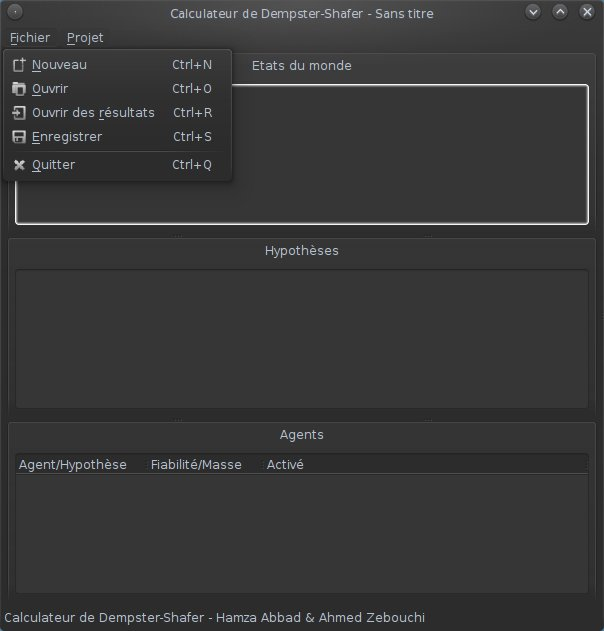
\includegraphics[width=\textwidth]{Inetrface_principale_menu_fichier}
\caption{Le menu \textbf{Fichier}}
\end{subfigure}
\hfill
\begin{subfigure}{0.49\textwidth}
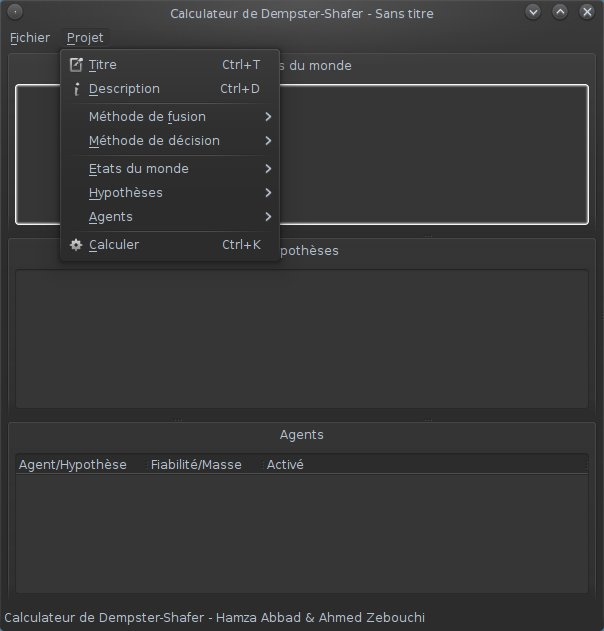
\includegraphics[width=\textwidth]{Inetrface_principale_menu_projet}
\caption{Le menu \textbf{Projet}}
\end{subfigure}
\caption{L'interface principale de la toolbox de Dempster-Shafer}
\end{figure}